\section{Conditional Heteroskedastic Models}\label{Conditional Heteroskedastic}
\paragraph{Primary Text Reading.} \citeA[chap. 3]{tsay2005aft}\index{Tsay, Ruey}

Up to this point, we have focused on modeling assets returns or forecasting their prices. When analyzing \fts{}, we may also want to analyze the \emph{volatility} or, the conditional standard deviation, of the asset. Since volatility is not directly experienced, we must find a substitute for it. We can look at an option pricing model that uses volatility as an input.

The \emph{implied volatility}\index{Implied volatility} of an option contract is the volatility implied by the market price of the option based on an option pricing model. It is the volatility that, given a particular pricing model, yields a theoretical value for the option equal to the current market price. Implied volatility, a forward-looking measure, differs from historical volatility because the latter is calculated from known past prices of a security.

One model, which requires conditional volatility as one of its inputs, is the Black-Scholes option pricing model,\index{Black-Scholes option pricing model}
\begin{subequations}
	\begin{eqnarray}
	C(S,T) &=& S\Phi(d_1) - Ke^{-rT}\Phi(d_2) \label{eq:bs-call} \\
	P(S,T) &=& Ke^{-rT}\Phi(-d_2) - S\Phi(-d_1) \label{eq:bs-put}
	\end{eqnarray}
\end{subequations}
where,
\begin{eqnarray*}
d_1 &=& \frac{\ln(S/K) + (r + \sigma^2/2)T}{\sigma\sqrt{T}} \notag \\
d_2 &=& d_1 - \sigma\sqrt{T} \notag \\
\Phi(\cdot) &=& \text{c.d.f. of the Normal Distribution, \eqref{eq:cdf}}. \notag
\end{eqnarray*}
Using this closed-form solution, we can obtain the price for either a call option \eqref{eq:bs-call} or a put option \eqref{eq:bs-put}\footnote{A \emph{call option} is a contract that gives the holder the right to \textbf{buy} a certain quantity of an underlying security from the writer of the option, at a specified price (the strike price) up to a specified date (the expiration date). 
A \emph{put option} is a contract that gives the holder the right to \textbf{sell} a certain quantity of an underlying security to the writer of the option, at a specified price up to a specified date.
}.
Similarly, if we have the option price, and all other inputs except the volatility, we can calculate the implied volatility by entering a value that would satisfy the equation. However, to do so may be relying upon the model (and its unrealistic assumptions) too much.

\paragraph{Volatility.} It is a difficult task to measure volatility of an asset return. Although the volatility may exist in a continuous form, with no sudden jumps, it may remain low for a period and then shift upward. Depending upon the asset, and whether it rose or fell in price, a major price change in the underlying security may affect volatility differently. To be certain, volatility changes, and it can be rapid and difficult to observe directly.

\margincomment[red]{Different volatility models make different assumptions about $\sigma^2_t$.}
To measure volatility, we need to model the changes in variance $\sigma^2_t$ in the asset return time series. The various conditional heteroskedastic models differ in how this variance changes in time. The evolution of $\sigma^2_t$ is deterministic in some models, such as the GARCH model, yet \emph{stochastic volatility}\index{Stochastic Volatility model} models exist also.

\subsection{Building a Volatility Model}
The basic structure of volatility modeling is
\[
r_t = \mu_t + a_t, \quad \mu_t = \phi_0 + \sum^k_{i=1}\beta_i x_{it} + \sum^p_{i=1}\phi_i r_{t-i}
- \sum^q_{i=1}\theta_i a_{t-i},
\]
and volatility models are concerned with time-evolution of
\[
\sigma^2_t = \text{Var} \left(r_t | F_{t-1} \right) = \text{Var} \left(a_t | F_{t-1} \right).
\]
Volatility model building requires four steps,
\begin{enumerate}
\item Create a mean equation and test for serial dependence in the \fts{}, and calibrate an AR or ARMA model to remove autocorrelation. For many asset returns, this is as simple as removing the sample mean from the data, and adding qualitative variables, as described in Section~\ref{dummy-variable}.
\item Test for ARCH effects with the residuals from the previous step.
\item If ARCH effects are statistically significant, choose a volatility model, and perform a joint estimation of the mean and volatility equations.
\item Refine the model if needed.
\end{enumerate}

\subsubsection{ARCH Effects}
If we denote $a_t = r_t - \mu_t$ as the residuals of the mean equation, then the squared series $a^2_t$ is used to check for conditional heteroskedacity. These are the \emph{ARCH effects}. There are two different tests available. We can apply the Ljung-Box statistic\index{Ljung-Box test} $Q(m)$ to  $\{a^2_t\}$ using as the null hypothesis that the first $m$ lags are zero. Another test is the \emph{Lagrange multiplier test}\index{Lagrange multiplier test}, which is equivalent to $F$ statistic for testing $\alpha_i=0 \quad (i=1,\ldots,m)$ in a linear regression
\[
a^2_t = \alpha_0 +\alpha_1 \alpha^2_{t-1}+\cdots+\alpha_m\alpha^2_{t-m}+e_t, \quad 
t=m+1,\ldots,T,
\]
where $e_t$ is the error term, $m$ is a specific positive integer, and $T$ is the sample size. The null hypothesis is $H_0: \alpha_1= \cdots a_m = 0$. Next, we need to define $SSR_0$ and $SSR_1$
\begin{eqnarray*}
SSR_0 &=& \sum^T_{t=m+1} (a^2_t - \bar{\omega})^2, \\
SSR_1 &=& \sum^T_{t=m+1} \hat{e}^2_t, 
\end{eqnarray*}
where $\bar{\omega}=(1/T)\sum^T_{t=1}a^2_t$ is the sample mean of $a^2_t$ and  $\hat{e}^t$ is the least squares residual of the prior linear regression. The $F$-test is then
\[
F=\frac{(SSR_0-SSR_1)/m}{SSR_1/(T-2m-1)}.
\]

\subsubsection{ARCH Model}
An \emph{autoregressive conditional heteroskedasticity} (ARCH) model\index{Autoregressive Conditional \\ Heteroskedasticity (ARCH) model} considers the variance of the current error term to be a function of the variances of the previous time period's error terms \cite{engle1982arch}.  ARCH relates the error variance to the square of a previous period's error. It is employed commonly in modeling financial time series that exhibit time-varying volatility clustering, which are periods of swings followed by periods of relative calm. The shock $a_t$ of an asset return is serially uncorrelated, but dependent; and the dependence can be described by a simple quadratic function of its lagged values.

%TODO: Maybe show asset returns and squared series for ARCH effect.

Specifically, let $\epsilon_t$  denote the returns (or return residuals, net of a mean process) and assume that $\epsilon_t=\sigma_t z_t$, where $z_t\sim iid~ N(0,1)$  and where the series $\sigma_t^2$  are modeled by
\[
\sigma_t^2=\alpha_0+\alpha_1 \epsilon_{t-1}^2+\cdots+\alpha_q \epsilon_{t-q}^2 = \alpha_0 + \sum_{i=1}^q \alpha_{i} \epsilon_{t-i}^2 
\]
and where $\alpha_0>0$  and $\alpha_i\ge 0,~i>0$.

\subsubsection{ARCH($q$) Model Specification}

An ARCH($q$) model can be estimated using ordinary least squares. A methodology to test for the lag length of ARCH errors using the Lagrange multiplier test was proposed by \citeA{engle1982arch}. Estimate the best fitting AR($q$) model
\[
y_t = a_0 + a_1 y_{t-1} + \cdots + a_q y_{t-q} + \epsilon_t = a_0 + \sum_{i=1}^q a_i y_{t-i} + \epsilon_t 
\]
Obtain the squares of the error $\hat{\epsilon}^2$  and regress them on a constant and $q$ lagged values,
\[
\hat \epsilon_t^2 = \hat \alpha_0 + \sum_{i=1}^{q} \hat \alpha_i \hat \epsilon_{t-i}^2
\]
where $q$ is the length of ARCH lags.

The null hypothesis is that, in the absence of ARCH effects, we have $\alpha_i = 0$ for all $i = \{1, \ldots, q\}$. The alternative hypothesis is that, in the presence of ARCH effects, at least one of the estimated $\alpha_i$ coefficients must be significant. In a sample of $T$ residuals under the null hypothesis of no ARCH errors, the test statistic $TR^2$ follows $\chi^2$ distribution with $q$ degrees of freedom. If $TR^2$ is greater than the chi-square table value, we reject the null hypothesis and conclude there is an ARCH effect in the ARMA model. If $TR^2$ is smaller than the chi-square table value, we accept the null hypothesis.

\paragraph{Model Building.}
%TODO: Test this code and expand on it.
Using the R library \texttt{FinTS}\index{FinTS@\texttt{FinTS} (library in R)}\footnote{Rmetrics has many other excellent functions in the \texttt{fSeries} package \cite{fseries-R}. A description of the many packages available from Rmetrics is at \texttt{http://www.rmetrics.org/rmetricsPackages.htm} and are available on CRAN.}
\cite{fints-R}, we can perform the Lagrange Multiplier (LM) test for autoregressive conditional heteroscedasticity (ARCH).
\ecaption{ARCH Test using R library, \texttt{FinTS}}
\begin{verbatim}
data(m.intc7303)
intcLM <- ArchTest(log(1+as.numeric(m.intc7303)), lag=12)
# Matches answer on Tsay (p. 102)
\end{verbatim}

\paragraph{Drawbacks of ARCH.} The ARCH model assume that positive and negative shocks have the same effect on volatility because it depends on the square of the previous shocks. This is not realistic. The ARCH model is not very helpful in finding the source of variation within a \fts{}. Also, the model responds slower to large isolated shocks.

\subsection{GARCH}\index{Generalized Autoregressive Conditional\\Heteroskedasticity (GARCH) model}\label{garch}
By comparison, ARCH models are simple, although the number of required parameters makes it difficult to calibrate. Next, we examine generalizations of ARCH to model volatility.
If an ARMA model is assumed for the error variance, the model is a generalized autoregressive conditional heteroskedasticity model \cite{bollerslev1986garch}. In such a case, the GARCH($m, s$) model, where $m$ is the order of the GARCH terms $\sigma^2$ and $s$ is the order of the ARCH terms $\epsilon^2$, is given by
\begin{eqnarray*}
\sigma_t^2&=&\alpha_0 + \alpha_1 \epsilon_{t-1}^2 + \cdots + \alpha_s \epsilon_{t-s}^2 + \beta_1 \sigma_{t-1}^2 + \cdots + \beta_m\sigma_{t-p}^2 \\
&=& \alpha_0 + \sum_{i=1}^q \alpha_i \epsilon_{t-i}^2 + \sum_{i=1}^m \beta_i \sigma_{t-i}^2.
\end{eqnarray*}
So that, the GARCH($m,s$) model is
\begin{equation}
a^2_t = \alpha_0 + \sum^{\max(m,s)}_{i=1} (\alpha_i + \beta_i) a^2_{t-i}+\eta_t
- \sum^s_{j=1} \beta_j \eta_{t-j}.
\label{eq:garch}
\end{equation}

\subsubsection{GARCH($m, s$) Model Specification}
The lag length $p$ of a GARCH process is established in three steps,
\begin{enumerate}
\item Estimate the best fitting AR($q$) model
\[
y_t = a_0 + a_1 y_{t-1} + \cdots + a_q y_{t-q} + \epsilon_t = a_0 + \sum_{i=1}^q a_i y_{t-i} + \epsilon_t 
\]
\item Compute and plot the autocorrelations of $\epsilon^2$ by 
\[
\rho = {{\sum^T_{t=i+1} (\hat \epsilon^2_t - \hat \sigma^2_t) (\hat \epsilon^2_{t-1} - \hat \sigma^2_{t-1})} \over {\sum^2_{t=1} (\hat \epsilon^2_t - \hat \sigma^2_t)^2}} 
\]
\item The asymptotic, large sample, standard deviation of $\rho(i)$ is $T^{-\frac{1}{2}}$. Individual values that are larger than this indicate GARCH errors. To estimate the total number of lags, use the Ljung-Box test until the value of the these are less than a 5\% significant. The Ljung-Box $Q$-statistic follows $\chi^2$ distribution with $n$ degrees of freedom if the squared residuals $\epsilon^2_t$  are uncorrelated. It is recommended to consider up to $T/4$ values of $n$. The null hypothesis states that there are ARCH or GARCH errors. Therefore, rejecting the null means that there are no such errors in the conditional variance.
\end{enumerate}

Specifying the order of a GARCH model is not easy, which is why lower order models such as GARCH(1,1), GARCH(1,2), or GARCH(2,1) are usually used. As long as the starting volatility is known, the conditional maximum likelihood method will work.

\paragraph{Forecasting with GARCH.}
Since volatility is not directly observable, testing and calibrating GARCH methods can be difficult. Often, one of the best ways to test a GARCH model for forecasting is to compare in-sample and out-of-sample results of volatility forecasts $\sigma^2_h(\ell)$ compared to shock $a^2_{h+\ell}$.

Forecasting with \eqref{eq:garch} can employ a similar method used when forecasting \eqref{eq:arma1-1}. Pursue the first parameter and seek the lowest AIC value, then hold that parameter constant while changing the second parameter. Sometimes, it may be helpful to go back and change the first parameter again after obtaining the second.

We can use a few R functions from the \texttt{fArma} library \cite{farma-R}, \texttt{fGarch} library \cite{fgarch-R}, and the \texttt{fSeries} library \cite{fseries-R} to examine GARCH models. The fit is displayed in Figure~\ref{figure:conditional-sd}.
\ecaption{GARCH Model Fitting in R}
\begin{verbatim}
spxm<-read.csv("SPX-M.csv", header=T)
spxts<-ts(spxm$Adj.Close, start=c(1950,1), frequency=12)
plot(spxts)

spxG<-garchFit(~garch(1, 1), data = spxts)
plot(spxG) # There are 13 different charts to choose from.
spxG@title
\end{verbatim}

With these functions, we can model the monthly volatility of the S\&P 500 Index with \texttt{fGarch}\index{fGarch@\texttt{fGarch} (library in R)} by starting with a GARCH(1,1) model. The \texttt{garchFit} function generates several statistics among its results,
\begin{verbatim}
Parameter Matrix:
                       U            V     params includes
    mu     -3.644376e+03     3644.376   364.4376     TRUE
    omega   1.968285e-01 19682849.836 19682.8498     TRUE
    alpha1  1.000000e-08        1.000     0.1000     TRUE
    gamma1 -1.000000e+00        1.000     0.1000    FALSE
    beta1   1.000000e-08        1.000     0.8000     TRUE
    delta   0.000000e+00        2.000     2.0000    FALSE
    skew    1.000000e-01       10.000     1.0000    FALSE
    shape   1.000000e+00       20.000     4.0000    FALSE
\end{verbatim}
Ultimately, after several iterations of changes in the log likelihood (``LLH''), we have a Hessian matrix,
\[
\begin{bmatrix}
      &          \mu  &    \omega   &  \alpha_1    &   \beta_1 \\
\mu    &   1.10102573  \\
\omega &   0.07283437 & 0.16546865 \\
\alpha_1 &  -0.28749874 & 0.98697087 & 311.6009165 \\
\beta_1 & -11.94005197 & 0 &  0  & -1.136868e+11
\end{bmatrix}.
\]

\pagebreak
We can examine the results graphically with 13 different types of graphs using \texttt{plot(spxG)}.  Between this and the statistics generated from the GARCH model, we can modify the parameter set $(m,s)$ for best fit.

\begin{footnotesize}
\begin{verbatim}
Make a plot selection (or 0 to exit): 

 1:   Time Series                                 2:   Conditional SD                           
 3:   Series with 2 Conditional SD Superimposed   4:   ACF of Observations                      
 5:   ACF of Squared Observations                 6:   Cross Correlation                        
 7:   Residuals                                   8:   Conditional SDs                          
 9:   Standardized Residuals                     10:   ACF of Standardized Residuals            
11:   ACF of Squared Standardized Residuals      12:   Cross Correlation between r^2 and r      
13:   QQ-Plot of Standardized Residuals          
\end{verbatim}
\end{footnotesize}

\begin{figure}[tb]
	\centering
	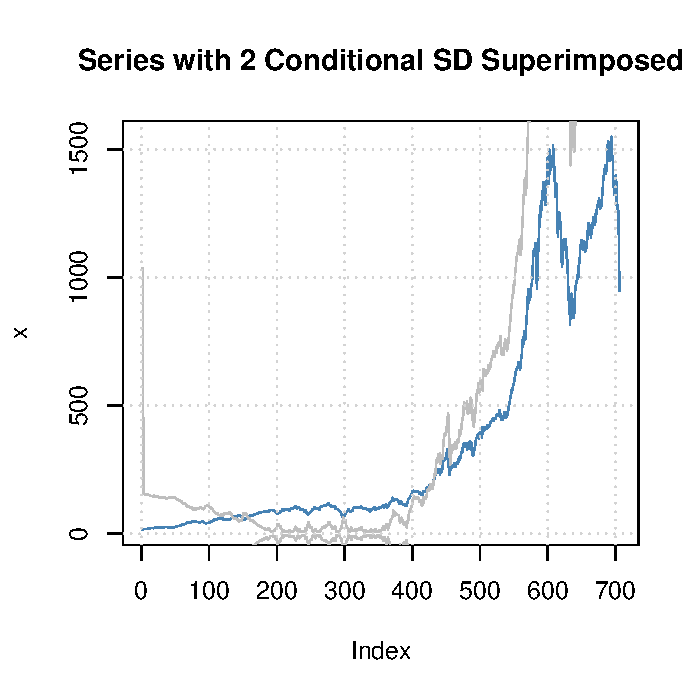
\includegraphics[scale=.8]{conditional-sd}
	\caption[S\&P 500 GARCH Estimate]{Monthly S\&P 500 GARCH Estimate with Two Conditional SD Superimposed}
	\label{figure:conditional-sd}
\end{figure}

\subsubsection{Integrated GARCH Model}\index{Integrated GARCH\\(IGARCH) model}
\margincomment[red]{IGARCH is a unit-root GARCH model.}
When AR polynomial of \eqref{eq:garch} has a unit root, then we have an IGARCH model.
The IGARCH(1,1) model
\begin{equation}
a_t = \sigma_t \epsilon_t, \quad \sigma^2_t = \alpha_0 + \beta_1 \sigma^2_{t-1} + (1-\beta_1)a^2_{t-1},
\label{eq:igarch}
\end{equation}
where $\{\epsilon_t\}$ is $1>\beta_1>0$. An IGARCH(1,1) model can be estimated by exponential smoothing methods when $\alpha_0=0$.

\subsubsection{GARCH in Mean Model}\index{GARCH in Mean\\(GARCH-M) model}
GARCH-M is a ``GARCH in the mean'' model because it adds the heteroskedastic term directly into the equation. It can be written as
\begin{eqnarray}
r_t &=& \mu + c\sigma^2_t + a_t, \quad a_t=\sigma_t \epsilon_t, \notag \\
\sigma^2_t &=& \alpha_0 + \alpha_1\alpha^2_{t-1} + \beta_1\sigma^2_{t-1},
\label{eq:garch-m}
\end{eqnarray}
where $\mu$ and $c$ are constants. The $c$ parameter is the \emph{risk premium parameter}. A $c>0$ indicates that the return has a positive relationship to its volatility.

\subsubsection{Exponential GARCH Model}\index{Exponential GARCH\\(EGARCH) model}
EGARCH was created to allow for asymmetric effects in asset returns. Positive and negative asset returns may not be equally symmetric, a problem not addressed by previous models. We begin with the weighted innovation
\[
g(\epsilon_t) = \theta \epsilon_t + \gamma \left[ |\epsilon_t| - E(|\epsilon_t|) \right],
\]
where $\theta$ and $\gamma$ are real constants. Both $\epsilon_t$ and $|\epsilon_t|-E(g(|\epsilon_t|)$ are zero-mean ($E[g(\epsilon_t)]$) iid sequences with continuous distributions. A better way to see the asymmetry is
\[
g(\epsilon_t) =
	\begin{cases}
	(\theta + \gamma)\epsilon_t - \gamma E(|\epsilon+t |) & \text{if $\epsilon_t \ge 0$,} \\
	(\theta - \gamma)\epsilon_t - \gamma E(|\epsilon+t |) & \text{if $\epsilon_t < 0$}.
	\end{cases}
\]
An EGARCH($m,s$) model can be written as
\begin{equation}
a_t = \sigma_t \epsilon_t, \quad \ln(\sigma^2_t)=\alpha_0 +
\frac{1+\beta_1 B+ \cdots +\beta_{s-1} B^{s-1}}{1-\alpha_1 B -\cdots -\alpha_m B^m} g(\epsilon_t - 1),
\label{eq:egarch}
\end{equation}
where $\alpha_0$ is a constant, $B$ is the \emph{back-shift} or lag operator such that $Bg(\epsilon_t)=g(\epsilon_{t-1})$, and $1+\beta_1 B +\cdots +\beta_{s-1} B^{s-1}$ and $1-\alpha_1 B -\cdots -\alpha_m B^m$ are polynomials with zeros outside the unit circle\footnote{To be \emph{outside the unit circle} means to have absolute values of the zeros greater than 1.} and have no common factors. The evolution of the conditional variance of $a_t$ is still contained in \eqref{eq:egarch} by using ARMA parameterization.

\paragraph{Alternative EGARCH Model.} An alternative form for EGARCH($m,s$) model is
\begin{equation}
\ln(\sigma^2_t) = \alpha_0 + \sum^s_{i=1} a_i \frac{|a_{t-i}|+\gamma_i a_{t-i}}{\sigma_{t-i}} +
\sum^m_{j=1} \beta_j \ln(\sigma^2_{t-j}).
\label{eq:egarch-alt}
\end{equation}
Notice in \eqref{eq:egarch-alt} that,
\begin{itemize}
\item a positive $a_{t-i}$ contributes $\alpha_i(1+\gamma_i)|\epsilon_{t-i}|$ to the log volatility,
\item a negative $a_{t-i}$ contributes $\alpha_i(1-\gamma_i)|\epsilon_{t-i}|$,
\end{itemize}
where $\epsilon_{t-i}=a_{t-i}/\sigma_{t-i}$. The leverage effect of $a_{t-i}$ is the $\gamma_i$ parameter.

\subsubsection{Conditional Heteroskedasticity (CHARMA) Model}\index{Conditional Heteroskedasticity\\(CHARMA) model}
The next model is CHARMA, which uses random coefficients to produce conditional heteroskedasticity. A CHARMA model is defined as
\begin{equation}
r_t = \mu_t + a_t, \quad a_t=\delta_{1t} a_{t-1} + \delta_{2t} a_{t-2} +\cdots +\delta_{mt} a_{t-m} + \eta_t,
\label{eq:charma}
\end{equation}
where $\{\eta_t\}$ is a Gaussian (normally distributed) white noise series with mean zero and variance $\sigma^2_{\eta}, \{\delta_t\}=\{(\delta_{1t}, \ldots,a_{mt})'\}$ is a sequence of iid random vectors with mean zero and non-negative definite covariance matrix $\mathbf{\Omega}$, and $\{\delta_t\}$ is independent of $\{\eta_t\}$.

The conditional variance of at of the CHARMA model \eqref{eq:charma} is
\begin{eqnarray}
\sigma^2_t &=& \sigma^2_{\eta} + \textbf{a}^{'}_{t-1} \text{Cov}(\delta)\textbf{a}_{t-1} \notag \\ 
&=& \sigma^2_t + (a, \ldots, a)\mathbf{\Omega}(a, \ldots, a).
\end{eqnarray}

\subsection{Stochastic Volatility Model}\index{Stochastic Volatility model}
If we model an underlying security's volatility as a random process, which is governed by state variables such as the price level of a security, there is a tendency of volatility to revert to some long-run mean value, and the variance of the volatility process itself.

Stochastic volatility models are one approach to resolve a shortcoming of some option pricing models that assume a fixed volatility during the life of the option contract. Because these option pricing models assume that the underlying volatility is constant over the life of the derivative, and unaffected by the changes in the price level of the underlying, they often misprice the option value. By assuming that the volatility of the underlying price is a stochastic process rather than a constant, it becomes possible to model derivatives more 
accurately.

The basic form of stochastic volatility is derived from Brownian motion, one of the simplest continuous-time stochastic processes, and is often used to model asset price movement.
\begin{equation}
dS_t = \mu S_t dt + \sigma S_t dW_t
\label{eq:brownian-motion}
\end{equation}

The maximum likelihood estimator to estimate the constant volatility $\sigma$, for given asset price time series $S_t$, at different times $t_i$, is 
\[
\hat{\sigma}^2= \left(\frac{1}{n} \sum_{i=1}^n \frac{(\ln S_{t_i}- \ln S_{t_{i-1}})^2}{t_i-t_{i-1}} \right) - \frac{1}{n} \frac{(\ln S_{t_n}- \ln S_{t_0})^2}{t_n-t_0}.
\]

\paragraph{GARCH Estimation.} The difficulty of estimating stochastic volatility is made slightly easier with GARCH methods, which assumes that the randomness of the variance process varies with the variance. The standard GARCH(1,1) model has this form for the variance differential
\[
d \nu_t = \theta(\omega - \nu_t )dt + \xi \nu_t dB_t .
\]

All stochastic volatility models have stochastic second moments (variance), but not all models that have stochastic second moments are called stochastic volatility models. Although stochastic volatility and GARCH are often presented as competing models, GARCH may help explain changes in volatility.

Both the ARCH/GARCH and stochastic volatility models derive their randomness 
from a white noise process. The difference is that an ARCH/GARCH process depends 
on just one white noise $W$. That white noise directly determines innovations in the ARCH/GARCH process while also indirectly determining innovations in its second moments. Despite the conventional description of \eqref{eq:brownian-motion}, stochastic volatility models generally depend on two white noise series, $V$ and $W$.

\paragraph{Heston model.} Another stochastic volatility model used for describing the evolution of the volatility of an underlying asset is the \emph{Heston model}\index{Heston model}. It assumes that the volatility of the asset is not constant, nor even deterministic, but follows a random process. Assuming that the asset price $S_t$ is determined by a stochastic process,
\[
dS_t = \mu S_t\,dt + \sqrt{\nu_t} S_t\,dW^S_t.
\]
The instantaneous variance is
\[
d\nu_t = \alpha(\theta - \nu_t)dt + \xi \sqrt{\nu_t}\,dW^{\nu}_t,
\]
where,
$\mu$ is the asset rate of return, $\theta$ is the long vol, or long run average price volatility; as $t$ tends to infinity, the expected value of $\nu_t$ tends to $\alpha$, $\alpha$ is the rate at which $\nu_t$ reverts to $\theta$, and $\xi$ is the volatility of the volatility (or, \emph{wiggle of the wiggle}), which determines the variance of $\nu_t$.
